\chapter{Cycles de vie et reproduction des plantes terrestres}\label{ch:b2:plant-life-cycles}

Le coussinet vert de \omterm{def:b2:plant-life-cycles:moss}{mousse} sur un mur est une plante~; les tiges brunes
qui s'en élèvent au printemps, portant chacune une capsule de spores,
en sont une autre --- un individu différent, avec deux fois plus de
chromosomes, qui pousse sur le premier et vit à ses dépens. Une fronde
de \omterm{def:b2:plant-life-cycles:fern}{fougère} porte des spores sur sa face inférieure, mais ces spores ne
donnent pas des \omterm{def:b2:plant-life-cycles:fern}{fougères}~: elles donnent une petite lame verte en forme
de cœur, large de quelques millimètres, où se forment les
spermatozoïdes et les oosphères, et c'est de cette lame que naît une
nouvelle \omterm{def:b2:plant-life-cycles:fern}{fougère}. Toute plante terrestre alterne ainsi entre deux
corps, l'un \omterm{def:b2:meiosis-heredity:meiosis}{haploïde} et l'autre \omterm{def:b2:meiosis-heredity:meiosis}{diploïde}. Ce chapitre suit cette
alternance des algues à la graine, et montre comment une succession de
modifications --- la réduction du corps \omterm{def:b2:meiosis-heredity:meiosis}{haploïde}, l'invention du \omterm{def:b2:plant-life-cycles:heterospory}{pollen},
l'enfermement de l'\omterm{def:b2:plant-life-cycles:heterospory}{ovule}, la graine --- a affranchi la reproduction de
l'eau et permis aux plantes de couvrir les continents.

\section{Trois types de cycles de vie}

\begin{definition}[Cycles haplophasique, diplophasique, haplodiplophasique]\label{def:b2:plant-life-cycles:cycles}
\index{cycle de vie}\index{alternance de generations@alternance de générations}\index{gametophyte}\index{sporophyte}
Tout cycle de vie sexué comprend une \emph{fécondation}, qui double le
nombre de chromosomes, et une \emph{\omterm{def:b2:meiosis-heredity:meiosis}{méiose}}, qui le divise par deux~;
les cycles diffèrent par ce qui se passe entre les deux. Dans un cycle
\emph{haplophasique}, le zygote est la seule cellule \omterm{def:b2:meiosis-heredity:meiosis}{diploïde} et subit
aussitôt la \omterm{def:b2:meiosis-heredity:meiosis}{méiose}~; l'organisme est \omterm{def:b2:meiosis-heredity:meiosis}{haploïde} et ses gamètes sont
produits par mitose (\emph{Chlamydomonas}, de nombreux champignons et
algues). Dans un cycle \emph{diplophasique}, la \omterm{def:b2:meiosis-heredity:meiosis}{méiose} produit
directement les gamètes, qui sont les seules cellules \omterm{def:b2:meiosis-heredity:meiosis}{haploïdes}, et
l'organisme est \omterm{def:b2:meiosis-heredity:meiosis}{diploïde} (les animaux, l'algue brune \emph{Fucus}).
Dans un cycle \emph{haplodiplophasique}, la \omterm{def:b2:meiosis-heredity:meiosis}{méiose} produit des
\emph{spores}, qui se développent par mitose en un organisme \omterm{def:b2:meiosis-heredity:meiosis}{haploïde},
le \emph{gamétophyte}, lequel produit des gamètes par mitose~; le
zygote se développe par mitose en un organisme \omterm{def:b2:meiosis-heredity:meiosis}{diploïde}, le
\emph{sporophyte}, qui produit des spores par \omterm{def:b2:meiosis-heredity:meiosis}{méiose}. Deux corps
\omterm{def:b2:unicellular-diversity:unicellular}{pluricellulaires} alternent --- c'est l'\emph{alternance de
générations} --- et c'est le cycle de toutes les plantes terrestres et
de nombreuses algues.
\end{definition}

\begin{omfigure}
\begin{tikzpicture}[every node/.style={font=\scriptsize}, >=stealth]
  \foreach \dx/\title/\hap/\dip in {0/{haplophasique (\emph{Chlamydomonas})}/{organisme haploïde ($n$)}/{zygote ($2n$)}, 5.2/{diplophasique (animaux)}/{gamètes ($n$)}/{organisme diploïde ($2n$)}, 10.4/{haplodiplophasique (plantes)}/{gamétophyte ($n$)}/{sporophyte ($2n$)}} {
    \begin{scope}[xshift=\dx cm]
      \node[anchor=south, font=\scriptsize\bfseries] at (2,2.5) {\title};
      \draw[thick, omDef, ->] (0.6,0.4) arc (200:340:1.5 and 1.0);
      \draw[thick, omThm, ->] (3.4,1.4) arc (20:160:1.5 and 1.0);
      \node[omDef, anchor=north] at (2,-0.3) {\hap};
      \node[omThm, anchor=south] at (2,2.05) {\dip};
      \node[anchor=south west] at (3.4,1.05) {fécondation};
      \node[anchor=north east] at (0.55,0.75) {méiose};
    \end{scope}
  }
  % emphasise the dominant phase by thickness of the arcs: draw thicker arcs
  \draw[line width=2.4pt, omDef, ->] (0.6,0.4) arc (200:340:1.5 and 1.0);
  \draw[line width=2.4pt, omThm, ->] (5.2+3.4,1.4) arc (20:160:1.5 and 1.0);
  \draw[line width=2.4pt, omDef, ->] (10.4+0.6,0.4) arc (200:340:1.5 and 1.0);
  \draw[line width=2.4pt, omThm, ->] (10.4+3.4,1.4) arc (20:160:1.5 and 1.0);
\end{tikzpicture}

{\small Trois \omterm{def:b2:plant-life-cycles:cycles}{cycles de vie}. En bleu~: la phase \omterm{def:b2:meiosis-heredity:meiosis}{haploïde}~; en rouge~: la
phase \omterm{def:b2:meiosis-heredity:meiosis}{diploïde}~; les arcs épais figurent les corps \omterm{def:b2:unicellular-diversity:unicellular}{pluricellulaires}.
Chaque cycle passe une fois par la \omterm{def:b2:meiosis-heredity:meiosis}{méiose} et une fois par la
fécondation~; ils diffèrent par la phase --- ou les deux --- qui se
développe en organisme.}
\end{omfigure}

\begin{proposition}[Ce que signifie l'alternance de générations]\label{prop:b2:plant-life-cycles:alternation}
Chez une plante terrestre, les deux générations sont deux organismes, et
non deux stades d'un même organisme~: le gamétophyte et le \omterm{def:b2:plant-life-cycles:cycles}{sporophyte}
ont des génomes différents (\omterm{def:b2:meiosis-heredity:meiosis}{haploïde} et \omterm{def:b2:meiosis-heredity:meiosis}{diploïde}), des corps différents,
des tailles souvent différentes de plusieurs ordres de grandeur, et
chacun se développe par mitose à partir d'une cellule unique --- une
spore ou un zygote. Le gamétophyte produit ses gamètes dans des organes
\omterm{def:b2:unicellular-diversity:unicellular}{pluricellulaires}, les \emph{\omterm{def:b2:plant-life-cycles:moss}{anthéridies}} (spermatozoïdes) et les
\emph{\omterm{def:b2:plant-life-cycles:moss}{archégones}} (une oosphère chacun, dans une bouteille dont le col
est descendu à la nage par le spermatozoïde)~; le \omterm{def:b2:plant-life-cycles:cycles}{sporophyte} produit
ses spores dans des \emph{\omterm{def:b2:plant-life-cycles:fern}{sporanges}}. D'un groupe de plantes terrestres
à l'autre, l'équilibre se déplace~: chez les \omterm{def:b2:plant-life-cycles:moss}{mousses}, le gamétophyte
est la plante et le \omterm{def:b2:plant-life-cycles:cycles}{sporophyte} une tige dépendante~; chez les \omterm{def:b2:plant-life-cycles:fern}{fougères},
le \omterm{def:b2:plant-life-cycles:cycles}{sporophyte} est la plante et le gamétophyte une lame autonome~; chez
les plantes à graines, le gamétophyte est réduit à quelques cellules
cachées dans les tissus du \omterm{def:b2:plant-life-cycles:cycles}{sporophyte} --- le grain de \omterm{def:b2:plant-life-cycles:heterospory}{pollen} et le
contenu de l'\omterm{def:b2:plant-life-cycles:heterospory}{ovule}.
\end{proposition}
\begin{proof}[Faits expérimentaux]
Hofmeister (1851) fit germer les spores de \omterm{def:b2:plant-life-cycles:moss}{mousses}, de \omterm{def:b2:plant-life-cycles:fern}{fougères}, de
prêles et de lycopodes, suivit le développement des petits corps verts
qu'elles produisaient, y trouva les \omterm{def:b2:plant-life-cycles:moss}{anthéridies} et les \omterm{def:b2:plant-life-cycles:moss}{archégones}, et
vit l'embryon se développer, à partir de l'oosphère fécondée à
l'intérieur de l'\omterm{def:b2:plant-life-cycles:moss}{archégone}, en plante porteuse de spores. Il montra
ensuite que l'\omterm{def:b2:plant-life-cycles:heterospory}{ovule} d'un conifère contient les mêmes structures,
réduites --- des \omterm{def:b2:plant-life-cycles:moss}{archégones} au sein d'un tissu qui est un gamétophyte
conservé --- et donc que \omterm{def:b2:plant-life-cycles:moss}{mousses}, \omterm{def:b2:plant-life-cycles:fern}{fougères} et plantes à graines forment
une seule série, avec un seul cycle. Les dénombrements de chromosomes
qui expliquèrent les deux générations (Strasburger, 1894) vinrent
quarante ans plus tard.
\end{proof}

\section{Les mousses~: le gamétophyte est la plante}

\begin{definition}[Le cycle de vie d'une mousse]\label{def:b2:plant-life-cycles:moss}
\index{mousse}\index{protonema@protonéma}\index{archegone@archégone}\index{antheridie@anthéridie}
Une \emph{spore} de mousse germe en un filament vert ramifié, le
\emph{protonéma}, sur lequel des bourgeons donnent les tiges feuillées
--- le \emph{gamétophyte}, haut de quelques centimètres, dépourvu de
vraies racines, de xylème et de phloème, ancré par des rhizoïdes et
absorbant l'eau par toute sa surface. À l'extrémité des tiges, il porte
des \emph{anthéridies}, qui libèrent des spermatozoïdes biflagellés dans
une pellicule de pluie ou de rosée, et des \emph{archégones}, contenant
chacun une oosphère à la base d'un col~; les spermatozoïdes nagent au
plus quelques centimètres, guidés par des substances attractives, et
fécondent l'oosphère sur place. Le zygote se développe en
\emph{\omterm{def:b2:plant-life-cycles:cycles}{sporophyte}}~: un pied enfoncé dans le gamétophyte, une tige
(la \emph{soie}) et une \emph{capsule} où la \omterm{def:b2:meiosis-heredity:meiosis}{méiose} produit des dizaines
de milliers de spores, libérées à travers une couronne de dents
hygroscopiques qui s'ouvrent à l'air sec. Le \omterm{def:b2:plant-life-cycles:cycles}{sporophyte} fait un peu de
photosynthèse, mais il est nourri par le gamétophyte à travers son pied
et ne vit jamais seul.
\end{definition}

\begin{omfigure}
\begin{tikzpicture}[every node/.style={font=\scriptsize}, >=stealth]
  \node[draw, rounded corners, fill=omDef!12, align=center] (spore) at (0,3) {spore ($n$)};
  \node[draw, rounded corners, fill=omDef!12, align=center] (proto) at (3.2,3) {protonéma};
  \node[draw, rounded corners, fill=omDef!12, align=center] (gam) at (6.6,3) {gamétophyte feuillé ($n$)\\anthéridies et archégones};
  \node[draw, rounded corners, fill=omDef!12, align=center] (gametes) at (11.2,3) {spermatozoïde et oosphère ($n$)};
  \node[draw, rounded corners, fill=omThm!12, align=center] (zyg) at (11.2,0.8) {zygote ($2n$)};
  \node[draw, rounded corners, fill=omThm!12, align=center] (sporo) at (6.6,0.8) {sporophyte ($2n$)\\pied, soie, capsule};
  \node[draw, rounded corners, fill=omThm!12, align=center] (cap) at (2.4,0.8) {méiose dans la capsule};
  \draw[->, thick] (spore) -- (proto) node[midway, above] {mitose};
  \draw[->, thick] (proto) -- (gam);
  \draw[->, thick] (gam) -- (gametes) node[midway, above] {mitose};
  \draw[->, thick] (gametes) -- (zyg) node[pos=0.3, right, align=left] {fécondation\\dans une pellicule d'eau};
  \draw[->, thick] (zyg) -- (sporo) node[midway, above] {mitose};
  \draw[->, thick] (sporo) -- (cap);
  \draw[->, thick] (cap) -| (spore) ;
  \node[omDef, anchor=west] at (-1.9,3.9) {haploïde};
  \node[omThm, anchor=west] at (-1.9,-0.1) {diploïde};
  \draw[gray, dashed] (-1.9,1.9) -- (13.2,1.9);
\end{tikzpicture}

{\small Le cycle d'une \omterm{def:b2:plant-life-cycles:moss}{mousse}. La plante feuillée est le gamétophyte
\omterm{def:b2:meiosis-heredity:meiosis}{haploïde}~; le \omterm{def:b2:plant-life-cycles:cycles}{sporophyte} est une tige et une capsule qui poussent sur
lui, nourries par lui, et qui produisent des spores par \omterm{def:b2:meiosis-heredity:meiosis}{méiose}.}
\end{omfigure}

\begin{omfigure}
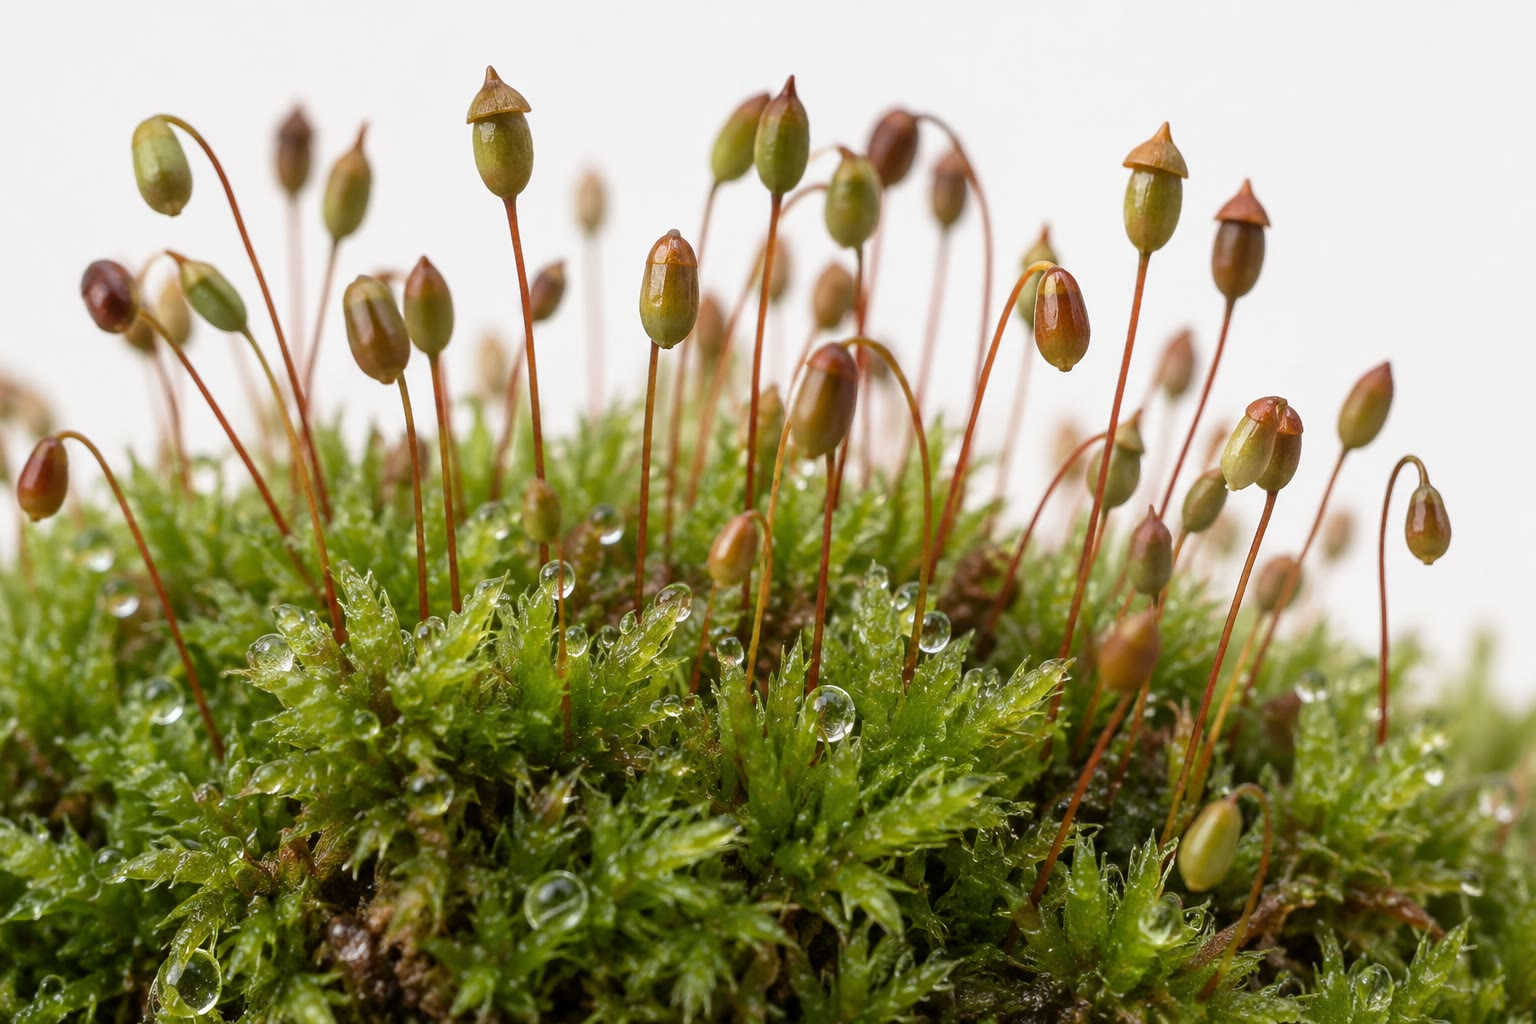
\includegraphics[width=0.6\linewidth]{images/book4/ai/b4-05-moss-sporophytes.jpg}

{\small Un coussinet de \omterm{def:b2:plant-life-cycles:moss}{mousse} au printemps~: les tiges vertes sont les
gamétophytes, et chaque tige rougeâtre portant sa capsule est un
\omterm{def:b2:plant-life-cycles:cycles}{sporophyte} issu d'une oosphère fécondée, encore attaché à la tige qui a
produit cette oosphère.}
\end{omfigure}

\begin{example}[Le coût des spermatozoïdes nageurs]\label{ex:b2:plant-life-cycles:sperm}
Un spermatozoïde de \omterm{def:b2:plant-life-cycles:moss}{mousse} nage à environ \qty{100}{\micro m/s}~; pour
atteindre un \omterm{def:b2:plant-life-cycles:moss}{archégone} situé à \qty{2}{cm}, il lui faut \qty{200}{s}
de pellicule d'eau continue --- une averse, une forte rosée. La
fécondation est donc limitée aux temps humides et aux courtes distances,
et la plupart des \omterm{def:b2:plant-life-cycles:moss}{mousses}, des \omterm{def:b2:plant-life-cycles:fern}{fougères} et de leurs parents vivent dans
des lieux humides ou se reproduisent à la saison des pluies~; chez
certaines \omterm{def:b2:plant-life-cycles:moss}{mousses}, les \omterm{def:b2:plant-life-cycles:moss}{anthéridies} sont logées dans une coupe dont la
forme projette à un demi-mètre les gouttes de pluie, et les
spermatozoïdes qu'elles emportent. C'est à cette dépendance que les
plantes à graines ont échappé.
\end{example}

\section{Les fougères~: le sporophyte est la plante}

\begin{definition}[Le cycle de vie d'une fougère]\label{def:b2:plant-life-cycles:fern}
\index{fougere@fougère}\index{prothalle}\index{sore}\index{sporange}
La fougère est le \emph{\omterm{def:b2:plant-life-cycles:cycles}{sporophyte}}~: un rhizome pourvu de racines, de
xylème et de phloème, et des frondes. Sous les frondes fertiles, des
groupes de \emph{sporanges} (les \emph{sores}, souvent recouverts d'un
repli protecteur) produisent chacun 64 spores par \omterm{def:b2:meiosis-heredity:meiosis}{méiose} et les
projettent par la détente d'un anneau de cellules à parois épaisses qui
se dessèche. Une spore tombée sur un sol humide se développe en
\emph{prothalle}~: un gamétophyte vert en forme de cœur, large de
quelques millimètres, épais d'une seule cellule, pourvu de rhizoïdes et
vivant librement pendant quelques semaines. Il porte des \omterm{def:b2:plant-life-cycles:moss}{anthéridies} et
des \omterm{def:b2:plant-life-cycles:moss}{archégones} sur sa face inférieure~; les spermatozoïdes nagent dans
la pellicule d'eau du sol jusqu'à l'oosphère~; le zygote se développe
en un jeune \omterm{def:b2:plant-life-cycles:cycles}{sporophyte} qui tire sa première nourriture du prothalle
puis s'enracine, et le prothalle meurt. Les deux générations sont
toutes deux autonomes, mais inégales~: le \omterm{def:b2:plant-life-cycles:cycles}{sporophyte} vit des décennies
et peut atteindre plusieurs mètres, le gamétophyte vit des semaines et
mesure quelques millimètres.
\end{definition}

\begin{omfigure}
\begin{tikzpicture}[every node/.style={font=\scriptsize}, >=stealth]
  \node[draw, rounded corners, fill=omThm!12, align=center] (fern) at (0,3) {fougère, le sporophyte ($2n$)\\racines, rhizome, frondes};
  \node[draw, rounded corners, fill=omThm!12, align=center] (sor) at (5.4,3) {sporanges groupés en sores\\(sous les frondes)};
  \node[draw, rounded corners, fill=omDef!12, align=center] (spore) at (10.4,3) {spores ($n$)\\64 par sporange};
  \node[draw, rounded corners, fill=omDef!12, align=center] (pro) at (10.4,0.6) {prothalle ($n$)\\autonome, millimétrique\\anthéridies, archégones};
  \node[draw, rounded corners, fill=omDef!12, align=center] (gam) at (5.4,0.6) {spermatozoïde et oosphère ($n$)};
  \node[draw, rounded corners, fill=omThm!12, align=center] (zyg) at (0,0.6) {zygote ($2n$), puis\\jeune sporophyte\\sur le prothalle};
  \draw[->, thick] (fern) -- (sor);
  \draw[->, thick] (sor) -- (spore) node[midway, above] {méiose};
  \draw[->, thick] (spore) -- (pro) node[midway, right] {mitose};
  \draw[->, thick] (pro) -- (gam) node[midway, above] {mitose};
  \draw[->, thick] (gam) -- (zyg) node[midway, above, align=center] {fécondation\\(spermatozoïdes nageurs)};
  \draw[->, thick] (zyg) -- (fern) node[midway, right] {mitose};
  \draw[gray, dashed] (7.9,-0.5) -- (7.9,4.0);
  \node[omThm, anchor=south] at (2.7,3.9) {génération diploïde};
  \node[omDef, anchor=south] at (10.4,3.9) {génération haploïde};
\end{tikzpicture}

{\small Le cycle d'une \omterm{def:b2:plant-life-cycles:fern}{fougère}. La plante que nous appelons \omterm{def:b2:plant-life-cycles:fern}{fougère} est
le \omterm{def:b2:plant-life-cycles:cycles}{sporophyte} \omterm{def:b2:meiosis-heredity:meiosis}{diploïde}~; le gamétophyte \omterm{def:b2:meiosis-heredity:meiosis}{haploïde} est un \omterm{def:b2:plant-life-cycles:fern}{prothalle}
éphémère sur lequel les spermatozoïdes nagent jusqu'aux oosphères.}
\end{omfigure}

\begin{omfigure}
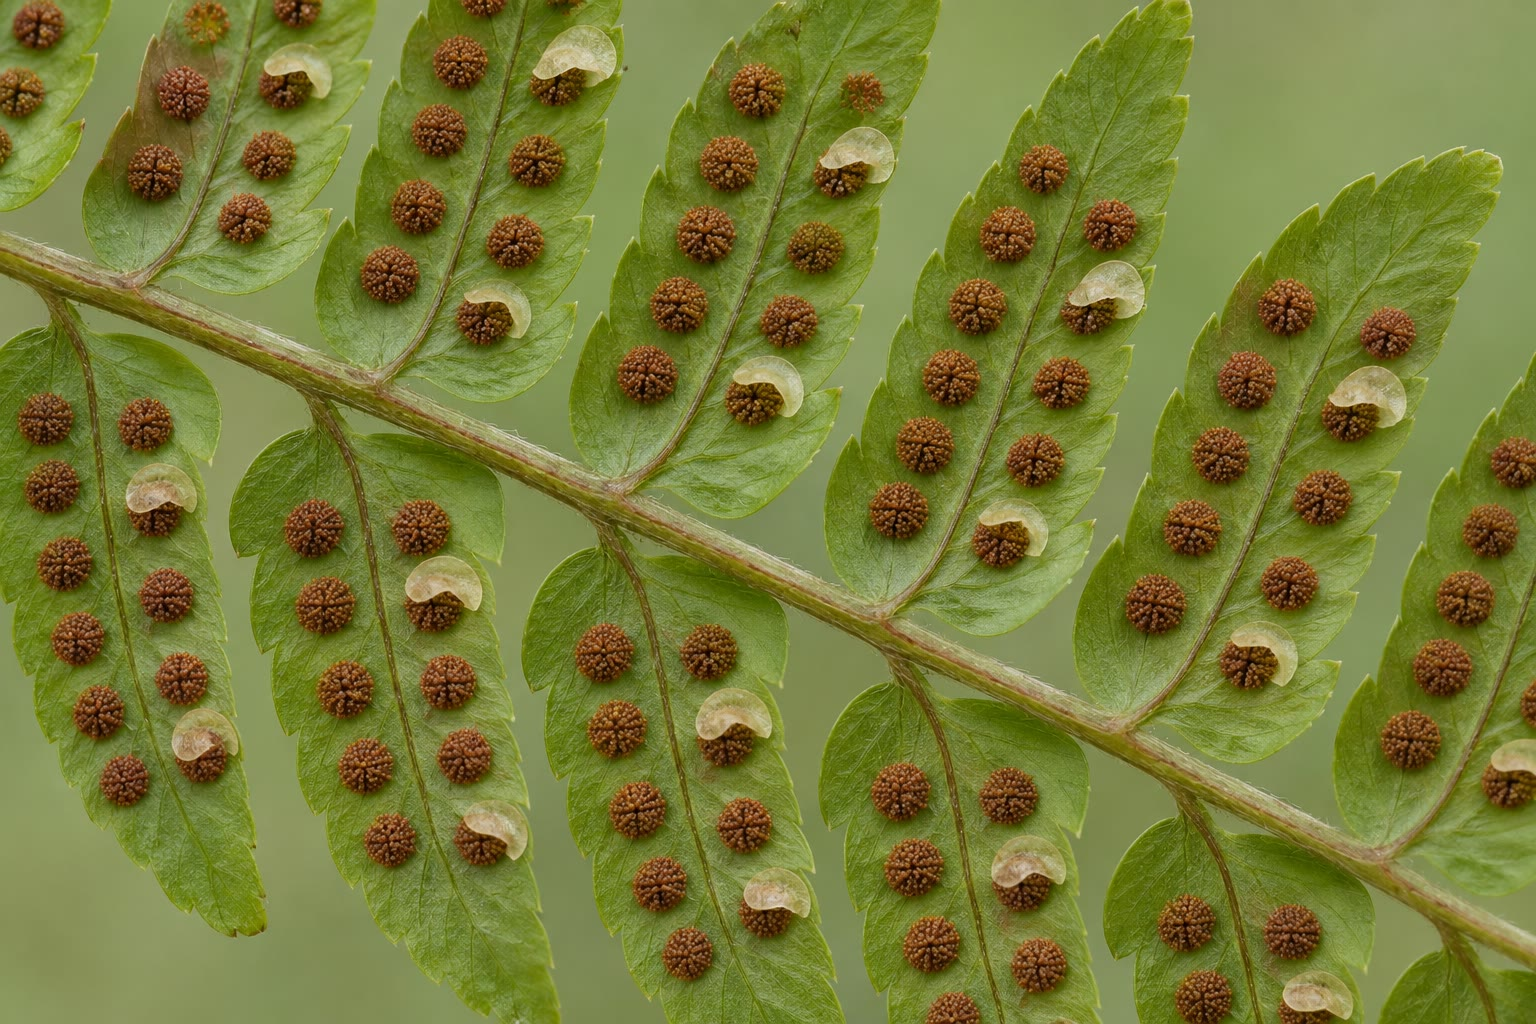
\includegraphics[width=0.6\linewidth]{images/book4/ai/b4-05-fern-sori.jpg}

{\small La face inférieure d'une fronde fertile de \omterm{def:b2:plant-life-cycles:fern}{fougère}~: chaque point
brun est un \omterm{def:b2:plant-life-cycles:fern}{sore}, un groupe de \omterm{def:b2:plant-life-cycles:fern}{sporanges}, dont certains sont encore
couverts par le repli qui les protège jusqu'à maturité.}
\end{omfigure}

\begin{theorem}[La dispersion d'une spore]\label{thm:b2:plant-life-cycles:dispersal}
\index{dispersion des spores}
Une spore de rayon $r$ et de masse volumique $\rho_s$, libérée à une
hauteur $h$ dans un vent horizontal de vitesse $u$, tombe à la vitesse
limite de Stokes
$v_s = 2r^2(\rho_s - \rho_{\text{air}})g/9\eta_{\text{air}}$
et atterrit, dans un air stratifié et calme, à une distance
\[
x = \frac{u\,h}{v_s}
\]
de la plante. Une spore de \omterm{def:b2:plant-life-cycles:fern}{fougère} de rayon \qty{15}{\micro m} et de
masse volumique \qty{1100}{kg/m^3} ($\eta_{\text{air}} = \qty{1.8e-5}{Pa.s}$)
tombe à \qty{3}{cm/s}~; depuis une fronde située à \qty{0.5}{m}, dans
un vent de \qty{2}{m/s}, elle parcourt environ \qty{30}{m}, et dans
l'air turbulent d'un jour de vent, qui soulève une fraction des spores
bien au-dessus de leur hauteur de libération, quelques-unes parcourent
des centaines de kilomètres --- ce qui explique que les flores de
\omterm{def:b2:plant-life-cycles:fern}{fougères} des îles océaniques soient riches et leurs flores de plantes à
graines pauvres.
\end{theorem}
\begin{proof}
La durée de la chute est $h/v_s$ (la spore atteint sa vitesse limite en
quelques microsecondes), pendant laquelle le vent la transporte de
$u\,h/v_s$. La vitesse limite s'obtient en équilibrant la traînée de
Stokes $6\pi\eta r
v_s$ et le poids diminué de la poussée d'Archimède $\tfrac43\pi r^3(\rho_s -
\rho_{\text{air}})g$, comme au \cref{ch:b2:unicellular-diversity}.
\end{proof}

\section{Les plantes à graines~: le gamétophyte est caché}

\begin{definition}[Hétérosporie, pollen, ovule]\label{def:b2:plant-life-cycles:heterospory}
\index{heterosporie@hétérosporie}\index{pollen}\index{ovule}\index{microspore}\index{macrospore}
Les \omterm{def:b2:plant-life-cycles:moss}{mousses} et la plupart des \omterm{def:b2:plant-life-cycles:fern}{fougères} sont \emph{isosporées}~: un seul
type de spore, un seul type de gamétophyte portant les deux sexes. Les
plantes à graines (et quelques \omterm{def:b2:plant-life-cycles:fern}{fougères} et lycopodes) sont
\emph{hétérosporées}~: les \emph{microspores}, petites et nombreuses,
se développent en gamétophytes mâles~; les \emph{macrospores}, grandes
et peu nombreuses, en gamétophytes femelles. Chez les plantes à graines,
les deux sont réduits presque à rien, et aucun ne quitte de lui-même les
tissus du \omterm{def:b2:plant-life-cycles:cycles}{sporophyte}. Le gamétophyte mâle est le \emph{grain de
pollen}~: une microspore qui s'est divisée deux ou trois fois à
l'intérieur de sa paroi, transportée par le vent ou par les animaux
jusqu'à l'organe femelle, où elle émet un \emph{tube pollinique} et
délivre ses gamètes mâles --- sans besoin d'eau. Le gamétophyte femelle
se développe à l'intérieur du macrosporange, qui reste sur la plante
mère, enveloppé d'un ou deux \emph{téguments} percés d'un pore, le
\emph{micropyle}~: l'ensemble est l'\emph{ovule}. Après la fécondation,
l'ovule devient la \emph{graine}~: un embryon de \omterm{def:b2:plant-life-cycles:cycles}{sporophyte}, une réserve
de nourriture et un tégument issu des téguments de l'ovule, en
dormance jusqu'à ce que les conditions soient favorables.
\end{definition}

\begin{omfigure}
\begin{tikzpicture}[every node/.style={font=\scriptsize}]
  % ovule in section
  \draw[thick, fill=omExo!25] (0,0) ellipse (1.6 and 2.2);
  \draw[thick, fill=omExo!10] (0,0) ellipse (1.25 and 1.85);
  \draw[thick, fill=white] (0,-0.15) ellipse (0.8 and 1.3);
  \draw[thick, fill=omDef!25] (0,0.6) ellipse (0.45 and 0.55);
  \fill[omDef!80!black] (0,0.75) circle (0.12);
  % micropyle: gap at top
  \fill[white] (-0.35,1.7) rectangle (0.35,2.35);
  \draw[thick] (-0.35,1.7) -- (-0.35,2.2); \draw[thick] (0.35,1.7) -- (0.35,2.2);
  \draw[thick] (-0.35,2.2) arc (180:90:0.1) ; \draw[thick] (0.35,2.2) arc (0:90:0.1);
  % pollen grain and tube
  \draw[thick, fill=omProp!40] (0.9,3.0) circle (0.22);
  \draw[thick, omProp] (0.75,2.85) .. controls (0.2,2.6) and (0.05,2.0) .. (0.05,1.25);
  % stalk
  \draw[thick] (0,-2.2) -- (0,-2.8);
  % labels
  \draw (1.45,-0.9) -- (2.6,-0.9) node[right] {tégument(s)};
  \draw (1.0,-0.6) -- (2.6,-1.5) node[right] {macrosporange (nucelle)};
  \draw (0.55,-1.0) -- (2.6,-2.1) node[right, align=left] {gamétophyte femelle\\(issu d'une macrospore)};
  \draw (0.35,0.45) -- (2.6,0.3) node[right] {archégone};
  \draw (0.1,0.78) -- (2.6,1.0) node[right] {oosphère};
  \draw (0.35,2.0) -- (2.6,2.0) node[right] {micropyle};
  \draw (1.1,3.0) -- (2.6,3.0) node[right] {grain de pollen et tube pollinique};
  \node[right] at (0.1,-2.6) {pédoncule};
\end{tikzpicture}

{\small Un \omterm{def:b2:plant-life-cycles:heterospory}{ovule} de gymnosperme en coupe. Le gamétophyte femelle, issu
d'une \omterm{def:b2:plant-life-cycles:heterospory}{macrospore} unique à l'intérieur du macrosporange, est enveloppé
d'un tégument percé d'un pore~; le grain de \omterm{def:b2:plant-life-cycles:heterospory}{pollen}, retenu au
micropyle, émet un tube jusqu'à l'oosphère. Après la fécondation,
l'ensemble devient la graine.}
\end{omfigure}

\begin{proposition}[Le cycle d'un conifère]\label{prop:b2:plant-life-cycles:conifer}
\index{conifere@conifère}\index{cone@cône}\index{graine}
Un pin porte deux sortes de cônes. Les petits \emph{cônes mâles},
groupés au printemps, contiennent des microsporanges où la \omterm{def:b2:meiosis-heredity:meiosis}{méiose}
produit des \omterm{def:b2:plant-life-cycles:heterospory}{microspores}~; chacune se divise en un grain de \omterm{def:b2:plant-life-cycles:heterospory}{pollen} de
quatre cellules muni de deux ballonnets et est libérée par millions
dans le vent. Les \emph{cônes femelles} portent deux \omterm{def:b2:plant-life-cycles:heterospory}{ovules} sur la face
supérieure de chaque écaille. Le \omterm{def:b2:plant-life-cycles:heterospory}{pollen} soufflé entre les écailles est
attiré jusqu'au micropyle par une gouttelette de liquide~; le
gamétophyte femelle, qui ne s'est pas encore développé, croît ensuite
pendant l'année suivante, à partir de la seule \omterm{def:b2:plant-life-cycles:heterospory}{macrospore} survivante,
en un tissu de quelques milliers de cellules portant deux ou trois
\omterm{def:b2:plant-life-cycles:moss}{archégones}~; un tube pollinique traverse lentement le nucelle et, quinze
mois après la pollinisation, délivre un gamète mâle à une oosphère.
L'embryon se développe dans le gamétophyte, qui devient la réserve
nutritive de la graine~; la graine, ailée, est libérée au deuxième
automne, lorsque le cône s'ouvre. Les graines demandent des années et
coûtent cher~; en retour, elles sont dispersées à l'état sec, survivent
à l'hiver et à la sécheresse, et emportent la nourriture des premières
semaines de la plantule.
\end{proposition}

\begin{omfigure}
\begin{tikzpicture}[every node/.style={font=\scriptsize}, >=stealth]
  \draw[thick, ->] (0,0) -- (13.2,0);
  \foreach \x/\l in {0/{printemps, année 1}, 4.4/{printemps, année 2}, 8.8/{automne, année 2}, 12.4/{}}
    \draw (\x,0.1) -- (\x,-0.1) node[below] {\l};
  \node[above, align=center, omProp] at (0.6,0.3) {pollinisation~:\\pollen retenu au micropyle};
  \node[above, align=center, omDef] at (3.0,1.2) {le gamétophyte femelle croît\\à partir de la macrospore (un an)};
  \draw[omDef, thick] (0.8,1.15) -- (5.2,1.15);
  \node[above, align=center, omThm] at (5.6,0.3) {fécondation~:\\le tube pollinique atteint l'oosphère};
  \node[above, align=center, omThm] at (8.2,1.2) {l'embryon se développe\\dans le gamétophyte};
  \draw[omThm, thick] (5.8,1.15) -- (10.4,1.15);
  \node[above, align=center] at (10.8,0.3) {le cône s'ouvre~:\\graines ailées libérées};
\end{tikzpicture}

{\small Le calendrier d'une graine de pin~: pollinisation au premier
printemps, fécondation plus d'un an après, libération de la graine au
deuxième automne --- environ dix-huit mois du \omterm{def:b2:plant-life-cycles:heterospory}{pollen} à la graine.}
\end{omfigure}

\begin{omfigure}
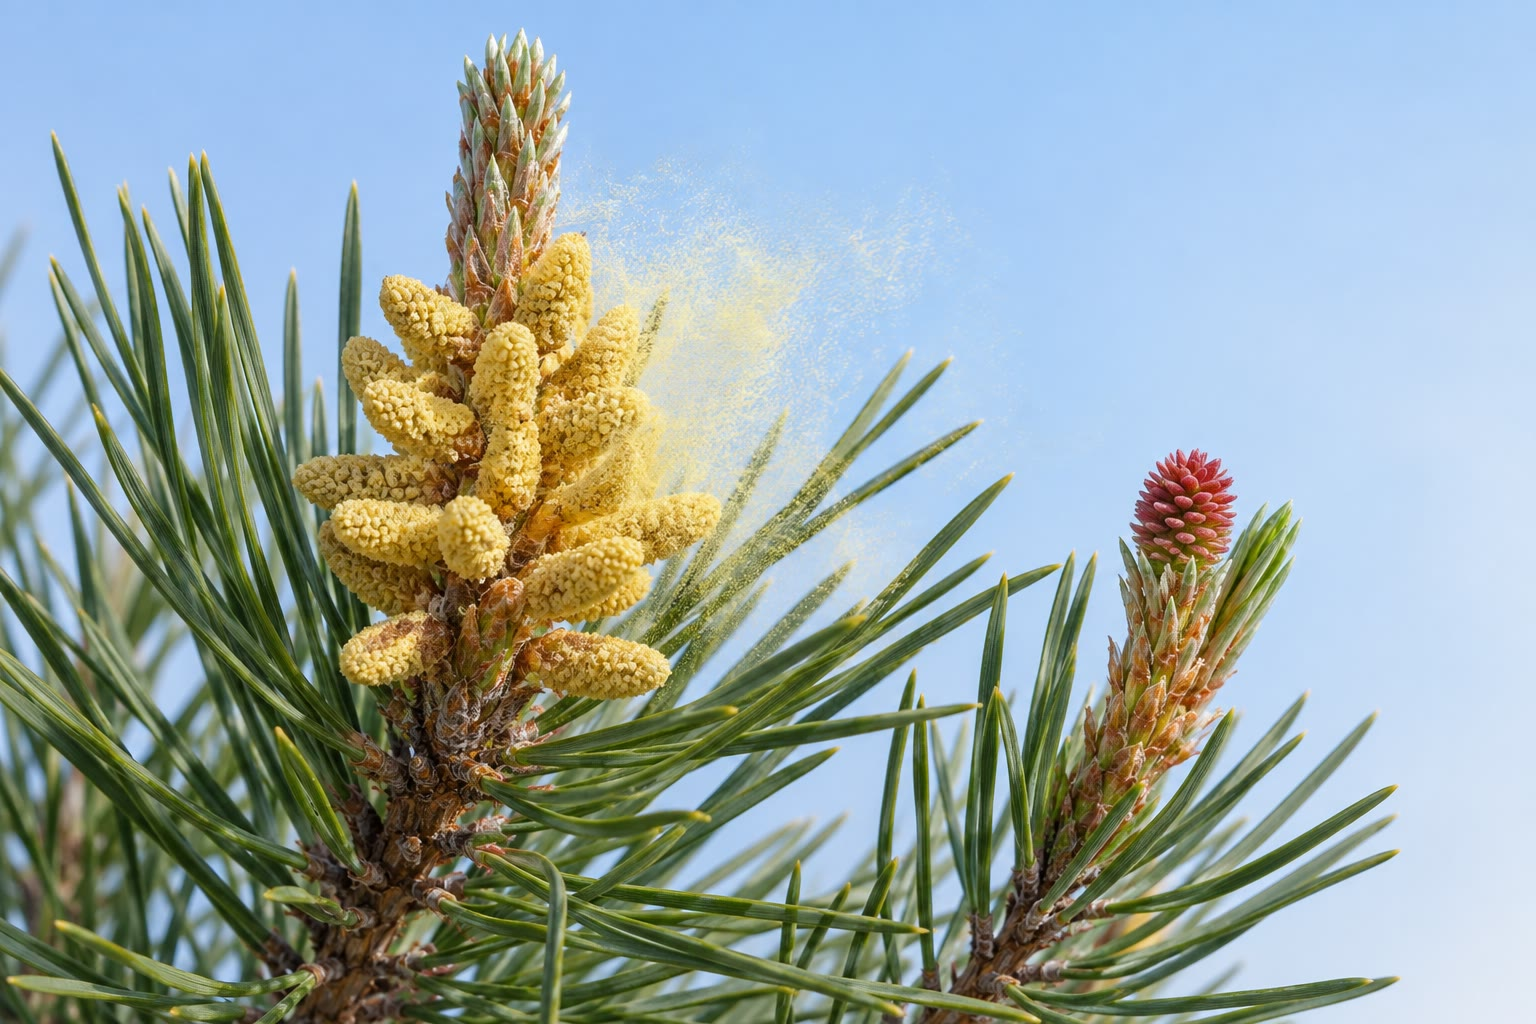
\includegraphics[width=0.6\linewidth]{images/book4/ai/b4-05-pine-cones.jpg}

{\small Une pousse de pin au printemps~: une grappe de cônes mâles jaunes
libérant leur \omterm{def:b2:plant-life-cycles:heterospory}{pollen}, et un petit cône femelle rouge à l'extrémité d'une
autre pousse, les écailles ouvertes pour le recueillir.}
\end{omfigure}

\begin{example}[Le pollen dans le vent]\label{ex:b2:plant-life-cycles:pollen}
Un grain de \omterm{def:b2:plant-life-cycles:heterospory}{pollen} de pin, de \qty{50}{\micro m} de diamètre et muni de
deux ballonnets, tombe à environ \qty{3}{cm/s}~; un grand arbre en
libère quelque
$10^{11}$ en une saison, de quoi couvrir les mares d'une pellicule
jaune. La probabilité qu'un grain donné tombe sur un \omterm{def:b2:plant-life-cycles:heterospory}{ovule} donné est
infime, et la stratégie ne fonctionne que par le nombre~: la
pollinisation par le vent est bon marché par grain, coûteuse en grains,
et réservée aux plantes qui poussent en peuplements de leur propre
espèce --- conifères, graminées, chênes. Les plantes à fleurs
(\cref{ch:b2:angiosperm-reproduction}) ont trouvé le moyen de faire
livrer le \omterm{def:b2:plant-life-cycles:heterospory}{pollen} par des animaux, grain par grain, à la bonne adresse.
\end{example}

\section{Tendances chez les plantes terrestres}

\begin{proposition}[Quatre tendances]\label{prop:b2:plant-life-cycles:trends}
\index{reduction du gametophyte@réduction du gamétophyte}
Des \omterm{def:b2:plant-life-cycles:moss}{mousses} aux \omterm{def:b2:plant-life-cycles:fern}{fougères} puis aux plantes à graines~: (1) le \omterm{def:b2:plant-life-cycles:cycles}{sporophyte}
passe d'une tige dépendante à la plante entière, et le gamétophyte se
réduit de la plante à une lame puis à quelques cellules~; (2)
l'isosporie cède la place à l'\omterm{def:b2:plant-life-cycles:heterospory}{hétérosporie}, et le gamétophyte femelle
reste sur la plante mère~; (3) la fécondation passe de spermatozoïdes
nageant dans l'eau de surface à un tube pollinique, si bien que la
reproduction n'a plus besoin de pluie~; (4) l'unité de dispersion passe
de la spore --- une cellule unique avec des réserves pour un jour --- à
la graine, un embryon pourvu de nourriture et d'un tégument, qui peut
attendre. La génération \omterm{def:b2:meiosis-heredity:meiosis}{diploïde} est favorisée sur la terre ferme parce
qu'un corps \omterm{def:b2:meiosis-heredity:meiosis}{diploïde} masque les \omterm{def:b2:genome-diversification:mutation}{mutations} récessives, peut, grâce à un
appareil vasculaire, devenir plus grand et vivre plus longtemps, et
parce qu'une spore produite par \omterm{def:b2:meiosis-heredity:meiosis}{méiose} sur un \omterm{def:b2:plant-life-cycles:cycles}{sporophyte} élevé voyage
plus loin qu'un gamète nageant depuis un gamétophyte bas. La tendance
se poursuit chez les plantes à fleurs, où le gamétophyte femelle compte
sept cellules et où la graine est enveloppée dans un fruit.
\end{proposition}

\begin{example}[Les groupes comparés]\label{ex:b2:plant-life-cycles:table}
\begin{center}
\small
\begin{tabular}{p{2.3cm}p{3.1cm}p{3.1cm}p{3.3cm}}
\hline
 & \omterm{def:b2:plant-life-cycles:moss}{mousses} & \omterm{def:b2:plant-life-cycles:fern}{fougères} & conifères \\
\hline
génération dominante & gamétophyte & \omterm{def:b2:plant-life-cycles:cycles}{sporophyte} & \omterm{def:b2:plant-life-cycles:cycles}{sporophyte} \\
gamétophyte & tige feuillée, cm & \omterm{def:b2:plant-life-cycles:fern}{prothalle}, mm, autonome & grain de \omterm{def:b2:plant-life-cycles:heterospory}{pollen} (4 cellules)~; contenu de l'\omterm{def:b2:plant-life-cycles:heterospory}{ovule} (des milliers de cellules) \\
spores & un seul type & un seul type & \omterm{def:b2:plant-life-cycles:heterospory}{microspores}, \omterm{def:b2:plant-life-cycles:heterospory}{macrospores} \\
fécondation & spermatozoïdes nageant dans l'eau & spermatozoïdes nageant dans l'eau & tube pollinique \\
unité de dispersion & spore & spore & graine \\
tissus conducteurs & aucun & xylème, phloème & xylème, phloème, bois \\
\hline
\end{tabular}
\end{center}
\end{example}

\section{Exercices}

\begin{exercise}[$\star$]\label{exo:b2:plant-life-cycles:1}
Définir gamétophyte, \omterm{def:b2:plant-life-cycles:cycles}{sporophyte}, spore et gamète, et indiquer par quel
type de division (mitose ou \omterm{def:b2:meiosis-heredity:meiosis}{méiose}) chacun des quatre est produit.
\end{exercise}

\begin{exercise}[$\star$]\label{exo:b2:plant-life-cycles:2}
La \omterm{def:b2:plant-life-cycles:fern}{fougère} \emph{Ophioglossum reticulatum} possède \num{1260}
chromosomes dans les cellules de ses feuilles. Combien en compte une
spore, une cellule de \omterm{def:b2:plant-life-cycles:fern}{prothalle}, un spermatozoïde, une oosphère, un
zygote~?
\end{exercise}

\begin{exercise}[$\star$]\label{exo:b2:plant-life-cycles:3}
À quelle génération appartient le coussinet vert d'une \omterm{def:b2:plant-life-cycles:moss}{mousse}~? La tige
brune portant une capsule~? Une fronde de \omterm{def:b2:plant-life-cycles:fern}{fougère}~? Un \omterm{def:b2:plant-life-cycles:fern}{prothalle}~? Un
grain de \omterm{def:b2:plant-life-cycles:heterospory}{pollen}~? La réserve nutritive d'une graine de pin~? L'embryon
d'une graine de pin~?
\end{exercise}

\begin{exercise}[$\star$]\label{exo:b2:plant-life-cycles:4}
Nommer les trois types de \omterm{def:b2:plant-life-cycles:cycles}{cycles de vie} et donner un organisme pour
chacun. Où la \omterm{def:b2:meiosis-heredity:meiosis}{méiose} a-t-elle lieu dans chacun d'eux~?
\end{exercise}

\begin{exercise}[$\star\star$]\label{exo:b2:plant-life-cycles:5}
Un spermatozoïde de \omterm{def:b2:plant-life-cycles:moss}{mousse} nage à \qty{100}{\micro m/s}. Combien de
temps met-il pour atteindre un \omterm{def:b2:plant-life-cycles:moss}{archégone} situé à \qty{3}{cm}~? Une
pellicule de rosée s'évapore \qty{20}{min} après le lever du soleil~:
quelle est la portée maximale de la fécondation~? Commenter la taille
des colonies de \omterm{def:b2:plant-life-cycles:moss}{mousses}.
\end{exercise}

\begin{exercise}[$\star\star$]\label{exo:b2:plant-life-cycles:6}
Calculer la vitesse de sédimentation dans l'air d'une spore de \omterm{def:b2:plant-life-cycles:fern}{fougère}
de rayon \qty{15}{\micro m} et de masse volumique \qty{1100}{kg/m^3}
($\eta =
\qty{1.8e-5}{Pa.s}$, $\rho_{\text{air}} = \qty{1.2}{kg/m^3}$), et la
distance qu'elle parcourt depuis \qty{0.5}{m} dans un vent de
\qty{2}{m/s}. Refaire le calcul pour une graine de pin de \qty{5}{mg}
dont l'aile lui donne une vitesse de descente de \qty{0.8}{m/s},
libérée depuis \qty{20}{m}.
\end{exercise}

\begin{exercise}[$\star\star$]\label{exo:b2:plant-life-cycles:7}
Une fronde de \omterm{def:b2:plant-life-cycles:fern}{fougère} porte \num{200} \omterm{def:b2:plant-life-cycles:fern}{sores} de \num{40} \omterm{def:b2:plant-life-cycles:fern}{sporanges},
chaque \omterm{def:b2:plant-life-cycles:fern}{sporange} produisant \num{64} spores. Combien de spores par
fronde~? Si une spore sur $10^{5}$ devient un \omterm{def:b2:plant-life-cycles:fern}{prothalle} et qu'un
\omterm{def:b2:plant-life-cycles:fern}{prothalle} sur \num{50} produit un \omterm{def:b2:plant-life-cycles:cycles}{sporophyte}, combien de jeunes
\omterm{def:b2:plant-life-cycles:fern}{fougères} une fronde fournit-elle~?
\end{exercise}

\begin{exercise}[$\star\star$]\label{exo:b2:plant-life-cycles:8}
Expliquer pourquoi l'\omterm{def:b2:plant-life-cycles:heterospory}{hétérosporie} est une condition préalable à la
graine, et pourquoi une plante isosporée ne pourrait pas enfermer son
gamétophyte femelle dans un \omterm{def:b2:plant-life-cycles:heterospory}{ovule}.
\end{exercise}

\begin{exercise}[$\star\star$]\label{exo:b2:plant-life-cycles:9}
Comparer une spore de \omterm{def:b2:plant-life-cycles:fern}{fougère} (une sphère de rayon \qty{15}{\micro m},
de masse volumique \qty{1100}{kg/m^3}) et une graine de pin
(\qty{5}{mg}) en tant qu'unités de dispersion~: masse, contenu
énergétique (prendre \qty{20}{kJ/g} de matière sèche, \qty{50}{\%} de
matière sèche), et ce que chacune peut et ne peut pas faire à
l'atterrissage.
\end{exercise}

\begin{exercise}[$\star\star\star$]\label{exo:b2:plant-life-cycles:10}
Un pin libère $10^{11}$ grains de \omterm{def:b2:plant-life-cycles:heterospory}{pollen} au-dessus d'une forêt~; à la
hauteur des \omterm{def:b2:plant-life-cycles:heterospory}{ovules}, les grains sont répartis dans une couche épaisse de
\qty{20}{m} sur \qty{1}{km^2}. Estimer la concentration du \omterm{def:b2:plant-life-cycles:heterospory}{pollen}
(grains par mètre cube), le nombre de grains par seconde qui traversent
l'ouverture micropylaire d'un \omterm{def:b2:plant-life-cycles:heterospory}{ovule} (\qty{0.1}{mm^2}) dans un vent de
\qty{2}{m/s}, et le temps nécessaire pour qu'un \omterm{def:b2:plant-life-cycles:heterospory}{ovule} reçoive un grain.
Qu'en déduire sur le moment de l'ouverture des cônes~?
\end{exercise}

\begin{exercise}[$\star\star\star$]\label{exo:b2:plant-life-cycles:11}
Donner trois raisons pour lesquelles la génération \omterm{def:b2:meiosis-heredity:meiosis}{diploïde} en est venue
à dominer le \omterm{def:b2:plant-life-cycles:cycles}{cycle de vie} des plantes terrestres, et une raison pour
laquelle la génération \omterm{def:b2:meiosis-heredity:meiosis}{haploïde} n'a pas complètement disparu.
\end{exercise}

\begin{exercise}[$\star\star\star$]\label{exo:b2:plant-life-cycles:12}
Hofmeister travailla avant que les chromosomes ne soient connus.
Expliquer ce qu'il pouvait et ne pouvait pas établir sur l'\omterm{def:b2:plant-life-cycles:cycles}{alternance de
générations} par la seule microscopie et la seule mise en culture, et ce
qu'apportèrent les dénombrements de chromosomes.
\end{exercise}

\section{Problème~: de la spore à la graine}

\begin{problem}[{Problème du week-end --- l'arithmétique reproductive d'une
fougère et d'un pin comparée, du nombre de spores et de grains de pollen
à leur dispersion, au devenir des gamétophytes et au coût d'une graine,
jusqu'au nombre de propagules que chaque plante doit produire pour se
remplacer une fois}]
\label{pb:b2:plant-life-cycles:1}
Une \omterm{def:b2:plant-life-cycles:fern}{fougère} porte \num{10} frondes fertiles, chacune avec \num{200}
\omterm{def:b2:plant-life-cycles:fern}{sores} de \num{40} \omterm{def:b2:plant-life-cycles:fern}{sporanges} produisant \num{64} spores chacun. Spores~:
rayon \qty{15}{\micro m}, masse volumique \qty{1100}{kg/m^3}. Un pin
produit au cours de sa vie les \omterm{def:b2:plant-life-cycles:heterospory}{ovules} de $2\times 10^{4}$ cônes femelles
--- prendre \num{100} \omterm{def:b2:plant-life-cycles:heterospory}{ovules} par cône --- et $10^{11}$ grains de \omterm{def:b2:plant-life-cycles:heterospory}{pollen}
par an. Graines~: \qty{5}{mg}, \qty{50}{\%} de matière sèche à
\qty{20}{kJ/g}. Air~: $\eta = \qty{1.8e-5}{Pa.s}$, $\rho =
\qty{1.2}{kg/m^3}$~; $g = \qty{9.81}{m/s^2}$.

\medskip
\noindent\textbf{Partie I --- Les spores de la \omterm{def:b2:plant-life-cycles:fern}{fougère}.}
\begin{enumerate}
  \item Calculer le nombre de spores que la plante libère en une saison.
  \item Calculer la masse d'une spore et celle de la récolte entière.
  \item Calculer la vitesse de sédimentation de la spore dans l'air.
  \item Depuis des frondes situées à \qty{0.5}{m}, dans un vent de
        \qty{1.5}{m/s}, quelle distance les spores parcourent-elles~? Sur
        quelle surface (un disque de ce rayon) sont-elles réparties, et
        combien en tombe-t-il par mètre carré~?
  \item Expliquer pourquoi la turbulence emporte quelques spores beaucoup
        plus loin, et ce que cela implique pour la colonisation d'une île
        nouvelle.
  \item Calculer le contenu énergétique d'une spore (\qty{50}{\%} de
        matière sèche à \qty{20}{kJ/g}) et celui de la récolte entière,
        et les comparer à l'énergie d'une graine de pin.
\end{enumerate}

\medskip
\noindent\textbf{Partie II --- Les gamétophytes.}
Une spore sur $2\times 10^{4}$ tombe sur un sol assez humide pour se
développer en \omterm{def:b2:plant-life-cycles:fern}{prothalle}~; un \omterm{def:b2:plant-life-cycles:fern}{prothalle} vit \num{6} semaines et a besoin
d'une nuit humide --- probabilité $0.2$ par semaine --- pour la
fécondation~; un \omterm{def:b2:plant-life-cycles:fern}{prothalle} fécondé donne un jeune \omterm{def:b2:plant-life-cycles:cycles}{sporophyte} avec une
probabilité de
$0.5$~; un jeune \omterm{def:b2:plant-life-cycles:cycles}{sporophyte} survit jusqu'à l'âge adulte avec une
probabilité de
$0.02$.
\begin{enumerate}[resume]
  \item Combien de \omterm{def:b2:plant-life-cycles:fern}{prothalles} la récolte de la plante produit-elle~?
  \item Calculer la probabilité qu'un \omterm{def:b2:plant-life-cycles:fern}{prothalle} connaisse au moins une
        nuit humide en six semaines.
  \item Calculer le nombre attendu de \omterm{def:b2:plant-life-cycles:fern}{fougères} adultes produites par la
        récolte d'une saison.
  \item Si la plante mère vit \num{30} ans, combien de descendants
        adultes laisse-t-elle, et qu'en déduire sur la population de
        \omterm{def:b2:plant-life-cycles:fern}{fougères}~?
  \item Un spermatozoïde de \omterm{def:b2:plant-life-cycles:fern}{fougère} nage à \qty{100}{\micro m/s}, et les
        \omterm{def:b2:plant-life-cycles:moss}{archégones} d'un \omterm{def:b2:plant-life-cycles:fern}{prothalle} se trouvent à \qty{1}{mm} de ses
        propres \omterm{def:b2:plant-life-cycles:moss}{anthéridies}. Combien de temps prend l'autofécondation~?
        Pourquoi de nombreuses \omterm{def:b2:plant-life-cycles:fern}{fougères} l'évitent-elles néanmoins
        (donner un mécanisme)~?
  \item En quel sens le \omterm{def:b2:plant-life-cycles:fern}{prothalle} est-il le maillon faible du cycle de
        la \omterm{def:b2:plant-life-cycles:fern}{fougère}~?
\end{enumerate}

\medskip
\noindent\textbf{Partie III --- Le \omterm{def:b2:plant-life-cycles:heterospory}{pollen} du pin.}
\begin{enumerate}[resume]
  \item Un grain de \omterm{def:b2:plant-life-cycles:heterospory}{pollen} est une sphère de rayon \qty{25}{\micro m} et
        de masse volumique effective \qty{600}{kg/m^3} (ballonnets
        compris). Calculer sa vitesse de sédimentation.
  \item Depuis un cône situé à \qty{15}{m}, dans un vent de
        \qty{3}{m/s}, quelle distance parcourt-il~?
  \item Les $10^{11}$ grains sont répartis sur \qty{1}{km^2} de forêt
        jusqu'à une hauteur de \qty{20}{m}. Calculer la concentration.
  \item Un micropyle présente une ouverture de \qty{0.1}{mm^2} à un vent
        de \qty{2}{m/s}. Calculer le nombre de grains qui y entrent par
        heure, et le temps nécessaire pour recevoir le premier grain.
  \item Expliquer pourquoi un pin isolé à \qty{5}{km} de la forêt ne
        produit presque aucune graine, et pourquoi les espèces
        pollinisées par le vent poussent en peuplements.
  \item Comparer les nombres~: combien de grains de \omterm{def:b2:plant-life-cycles:heterospory}{pollen} la forêt
        produit-elle par \omterm{def:b2:plant-life-cycles:heterospory}{ovule}, si elle compte \num{1000} pins portant
        chacun \num{2000} \omterm{def:b2:plant-life-cycles:heterospory}{ovules}~?
\end{enumerate}

\medskip
\noindent\textbf{Partie IV --- Les graines du pin.}
Parmi les \omterm{def:b2:plant-life-cycles:heterospory}{ovules} de l'arbre, \qty{60}{\%} sont pollinisés et
\qty{80}{\%} de ceux-ci forment une graine pleine~; une graine devient
une plantule avec une probabilité de $0.05$, et une plantule un adulte
avec une probabilité de $0.01$.
\begin{enumerate}[resume]
  \item Calculer le nombre de graines que l'arbre produit au cours de sa
        vie, ainsi que leur masse et leur énergie totales.
  \item Une graine ailée descend à \qty{0.8}{m/s}. Depuis \qty{20}{m},
        dans un vent de \qty{3}{m/s}, quelle distance parcourt-elle~?
        Comparer au \omterm{def:b2:plant-life-cycles:heterospory}{pollen}.
  \item Calculer le nombre attendu de descendants adultes, et le
        comparer à celui de la \omterm{def:b2:plant-life-cycles:fern}{fougère}.
  \item Calculer l'énergie que l'arbre investit par descendant adulte,
        et celle que la \omterm{def:b2:plant-life-cycles:fern}{fougère} investit par descendant adulte (spores
        seulement), et les comparer.
  \item La spore de \omterm{def:b2:plant-life-cycles:fern}{fougère} peut attendre quelques semaines~; la graine
        de pin plusieurs années. Expliquer, à l'aide des chiffres
        d'énergie, pourquoi la graine peut se permettre la dormance et
        la spore non.
  \item Donner deux avantages qui justifient le coût de la graine, et
        deux conditions dans lesquelles la stratégie de la \omterm{def:b2:plant-life-cycles:fern}{fougère} est la
        meilleure.
  \item Énoncer le résultat~: le nombre de propagules par descendant
        adulte pour la \omterm{def:b2:plant-life-cycles:fern}{fougère} et pour le pin, et l'énergie que chacun
        dépense par descendant adulte.
\end{enumerate}
\end{problem}
